\item \textbf{{[}DHS/PRELIM/9597/2019/P1/Q4{]} }

The Viola-Jones object detection algorithm, named after two computer
vision researchers Paul Viola and Michael Jones, uses integral images
to detect the presence of facial features in an image efficiently. 

An integral image (also known as a summed-area table) is the name
of both a data structure and an algorithm used to obtain this data
structure. It uses a quick and efficient way to calculate the sum
of pixel values in a rectangular part of an image. 

In an integral image, the value of each point is the sum of all pixels
above and to the left, including the target pixel: 
\begin{center}
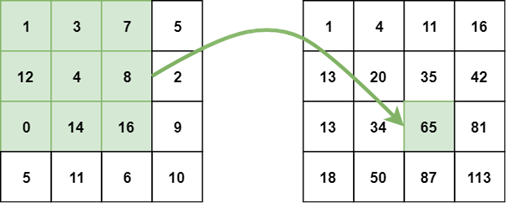
\includegraphics[width=0.5\paperwidth]{C:/Users/Admin/Desktop/Github/question_bank/LyX/static/img/9597-DHS-2019-P1-Q4-1}
\par\end{center}

The integral image can be calculated in a single pass over the original
image. This reduces summing the pixel intensities within a rectangle
into only three operations with four numbers, regardless of rectangle
size: 
\begin{center}
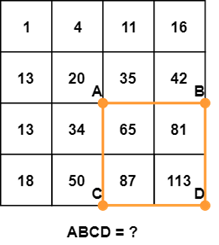
\includegraphics[width=0.25\paperwidth]{C:/Users/Admin/Desktop/Github/question_bank/LyX/static/img/9597-DHS-2019-P1-Q4-2}
\par\end{center}

The sum of pixels in the rectangle ABCD can be derived from the values
of points A, B, C, and D, using the formula $D-B-C+A$. It is easier
to understand this formula visually:

Note that subtracting both B and C means that the area defined with
A has been subtracted twice, so we need to add it back again. 

Thus $D-B-C+A=113-50-42+20=41$. 
\begin{center}
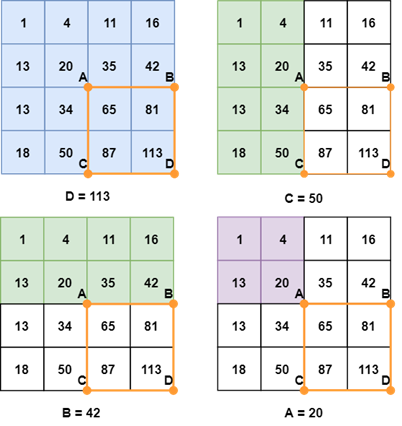
\includegraphics[width=0.5\paperwidth]{C:/Users/Admin/Desktop/Github/question_bank/LyX/static/img/9597-DHS-2019-P1-Q4-3}
\par\end{center}

\subsection*{Task 4.1 }

Write an \texttt{integral\_image()} function which reads in the data
from the file \texttt{IMAGE1.IN} into a 2D array and computes and
outputs the integral image to a file \texttt{IMAGE1.OUT} using the
algorithm described above, and also displays the result of $D-B-C+A$
to the screen. 

\subsection*{Evidence 19}

Program code. \hfill{} {[}13{]}

\subsection*{Evidence 20}

Screenshots of \texttt{IMAGE1.OUT} and output of $D-B-C+A$. \hfill{}{[}2{]}

\subsection*{Task 4.2}

Write a \texttt{magic()} function which is a generalisation of your
\texttt{integral\_image()} function which will work for any $m\times n$
rectangular 2D array and any rectangle ABCD.

Programmatically randomise your image with suitable values ($m,n\geq8$)
in \texttt{IMAGE2.IN} and work your magic on this pseudo-randomly
generated file to produce \texttt{IMAGE2.OUT} and the updated computed
value of $D-B-C+A$. 

\subsection*{Evidence 21}

Program code. \hfill{}{[}13{]}

\subsection*{Evidence 22 }

Screenshots of \texttt{IMAGE2.OUT} and output of $D-B-C+A$. \hfill{}{[}2{]}